% Opcje klasy 'iithesis' opisane sa w komentarzach w pliku klasy. Za ich pomoca
% ustawia sie przede wszystkim jezyk i rodzaj (lic/inz/mgr) pracy, oraz czy na
% drugiej stronie pracy ma byc skladany wzor oswiadczenia o autorskim wykonaniu.
\documentclass[inz,shortabstract]{iithesis}
% Własne dodatkowe pakiety:
\usepackage{graphicx}
\usepackage{float}
\usepackage[utf8]{inputenc}
\usepackage{listings}
\usepackage{xcolor}
\newcommand{\ind}{\\\indent}
\newcommand{\ap}{,,Implementacja narzędzia rozszerzającego usługę Google Forms''}
\colorlet{punct}{red!60!black}
\definecolor{background}{HTML}{EEEEEE}
\definecolor{delim}{RGB}{20,105,176}
\colorlet{numb}{magenta!60!black}

\lstdefinelanguage{json}{
    basicstyle=\normalfont\ttfamily,
    numbers=left,
    numberstyle=\scriptsize,
    stepnumber=1,
    numbersep=8pt,
    showstringspaces=false,
    breaklines=true,
    frame=lines,
    backgroundcolor=\color{background},
    literate=
     *{0}{{{\color{numb}0}}}{1}
      {1}{{{\color{numb}1}}}{1}
      {2}{{{\color{numb}2}}}{1}
      {3}{{{\color{numb}3}}}{1}
      {4}{{{\color{numb}4}}}{1}
      {5}{{{\color{numb}5}}}{1}
      {6}{{{\color{numb}6}}}{1}
      {7}{{{\color{numb}7}}}{1}
      {8}{{{\color{numb}8}}}{1}
      {9}{{{\color{numb}9}}}{1}
      {:}{{{\color{punct}{:}}}}{1}
      {,}{{{\color{punct}{,}}}}{1}
      {\{}{{{\color{delim}{\{}}}}{1}
      {\}}{{{\color{delim}{\}}}}}{1}
      {[}{{{\color{delim}{[}}}}{1}
      {]}{{{\color{delim}{]}}}}{1},
}

%% Makra dla tytułów, które pojawiają się także w streszczeniu

%%%%% DANE DO STRONY TYTUŁOWEJ
% Niezaleznie od jezyka pracy wybranego w opcjach klasy, tytul i streszczenie
% pracy nalezy podac zarowno w jezyku polskim, jak i angielskim.
% Pamietaj o madrym (zgodnym z logicznym rozbiorem zdania oraz estetyka) recznym
% zlamaniu wierszy w temacie pracy, zwlaszcza tego w jezyku pracy. Uzyj do tego
% polecenia \fmlinebreak.
\polishtitle    {Rozwój narzędzia rozszerzającego\fmlinebreak usługę Google Forms}
\englishtitle   {Development of an extension to Google Forms service}
\polishabstract {Praca jest kontynuacją pracy Agnieszki Pawickiej 
,,Implementacja narzędzia rozszerzającego usługę Google Forms''. Zawiera 
implementację oraz opis rozwijanego rozszerzenia do usługi Google Forms.
Rozszerzenie to pozwala na automatyczne generowanie formularzy
z odpowiedniego pliku w formacie JSON, konwertowanie wstawek matematycznych
napisanych w \LaTeX{} do odpowiednich symboli oraz zarządzanie niektórymi
własnościami utworzonych uprzednio formularzy. W pracy znajduje się również
omówienie wykorzystanych technologii.
}
\englishabstract{}

% w pracach wielu autorow nazwiska mozna oddzielic poleceniem \and
\author         {Aleksandra Rozkrut}
% w przypadku kilku promotorow, lub koniecznosci podania ich afiliacji, linie
% w ponizszym poleceniu mozna zlamac poleceniem \fmlinebreak

\advisor        {dr hab. Jan Otop, prof. UWr}
\date          {Wrocław 2022}
% Dane do oswiadczenia o autorskim wykonaniu
\transcriptnum {299745}                     % Numer indeksu
\advisorgen    {dr hab. Jana Otopa, prof. UWr} % Nazwisko promotora w dopelniaczu
%%%%%

\begin{document}
%%%%% POCZĄTEK ZASADNICZEGO TEKSTU PRACY
\chapter{Wprowadzenie}%Wstęp - opis problemu, motywacja

Wraz z rozpoczęciem pandemii problem zdalnego sprawdzania wiedzy i umiejętności
 zrobił się popularny. Miejsca, w których było to szczególnie uciążliwe to m.~in. szkoły, 
uczelnie, czy procesy rekrutacyjne w różnych firmach. Dobre narzędzie do przeprowadzania zdalnych
testów powinno spełniać pewne wymagania, takie jak:
\begin{itemize}
  \item przejrzystość formularzy,
  \item łatwość tworzenia nowych testów,
  \item możliwość skutecznego weryfikowania tożsamości osoby piszącej test.
\end{itemize}
\\Dodatkowo dobrze jest, gdy takie narzędzie posiada również takie funkcje jak:
\begin{itemize}
  \item automatyczne sprawdzanie pytań zamkniętych,
  \item kontrolowanie czasu potrzebnego poszczególnym osobom na zakończenie testu,
  \item możliwość losowych zmian kolejności pytań,
  \item możliwość zapisywania odpowiedzi w popularnym formacie.
\end{itemize}
\\Ponadto niektórzy egzaminujący cenią sobie możliwość wstawiania symboli matematycznych, 
wykresów czy zdjęć w ramach pytań.

\\ We wrześniu 2021 roku Agnieszka Pawicka obroniła pracę inżynierską o tytule \ap, 
 w której zaproponowała system umożliwiający generowanie testów Google Form z pliku 
 w formacie JSON. Projekt umożliwiał także generowanie pytań zawierająch wstawki w \LaTeX, 
 które były automatycznie kompilowane i wstawiane do formularza.
 \\ Celem tej pracy jest usprawnienie działania wymienionego wyżej narzędzia.
 \section{Wprowadzone usprawnienia}
W pracy został zaimplementowany szereg modyfikacji, które ułatwiają korzystanie z narzędzia
zarówno przy tworzeniu formularzy, zarządzaniu nimi, jak i ich późniejszym sprawdzaniu. Te usprawnienia to:
\begin{itemize}
  \item łatwiejszy sposób instalacji narzędzia,
  \item zmiana interfejsu użytkownika na bardziej intuicyjny,
  \item zmiana sposobu wgrywania zakodowanego formularza,
  \item możliwość edycji pliku JSON z zakodowanym formularzem już po wgraniu go,
  \item możliwość zobaczenia odpowiedzi oraz wyników w formacie JSON,
  \item możliwość pobrania danych o przesłanych odpowiedziach 
   i wynikach sprawdzania automatycznego w formacie EXCEL,
  \item utworzone formularze są teraz przechowywane na Dysku Google użytkownika 
  - nie jak w poprzedniej wersji na wspólnym dysku dla wszystkich użytkowników,
  \item szereg nowych opcji związanych z parametrami formularza tj.:
  \begin{itemize}
    \item możliwość zmiany kolejności odpowiedzi wewnątrz pytań zamknietych,
    \item możliwość dodania  opisu testu,
    \item odpowiedzi do pytań mogą być teraz w formie symboli  matematycznych (\LaTeX),
    \item możliwe jest dodanie oceniania innego niż zerojedynkowe dla pytań
     wielokrotnego wyboru.
  \end{itemize}  
\end{itemize}

\\Wszystkie wymienione zmiany wraz z użytymi narzędziami, instrukcją użytkownika oraz opisem
środowsk i napotkanych problemów są opisane w dalszych rozdziałach niniejszej pracy. 


\chapter{Środowisko}
Praca jest rozszerzeniem innego projektu, wobec tego część użytych bibliotek zostało opisanych 
w rozdziale ,,Środowisko'' pracy \ap. W niniejszym rozdziale skupię się więc na nowo dodanych
elementach środowiska. W celu zapoznania się z całością polecam lekturę wymienionej 
pracy.
\\ Kod projektu można podzielić na cztery główne części:
\begin{enumerate}
  \item interfejs użytkownika,
  \item serwer komunikujący się z zewnętrznymi API oraz bazą danych,
  \item kod służący do instalacji zależności i uruchamiania aplikacji na maszynie wirtualnej 
  - korzystający z technologii Vagrant i Ansible
  \item skrypt w języku Python konwertujący wstawki w języku \LaTeX\ do obrazów.
\end{enumerate}
Dodatkowo aplikacja korzysta z Google Forms API oraz Imgur API.

\section{Interfejs użytkownika}

\subsection{TypeScript}
Aplikacja została napisana w języku TypeScript, który jest nadzbiorem języka JavaScript. 
Aplikacja korzysta z bibliotek: 
types/node, typescript.

\subsection{React}
Technologia służąca do tworzenia interfejsów
graficznych aplikacji internetowych. Aplikacja korzysta z bibliotek:
emotion/react, emotion/styled, types/react, types/react-dom, 
react, react-dom, react-scripts.

\subsection{Material UI}
Biblioteka udostępniająca wiele gotowych komponentów, których można użyć w~
aplikacjach korzystających z Reacta. 

\subsection{axios}
Biblioteka służąca do wysyłania zapytań http i pobierania danych z serwera.

\subsection{date-fns}
Biblioteka pomagająca zarządzać datami. Udostępnia wiele użytecznych funkcji.

\subsection{react-code-blocks}
Biblioteka z gotowymi komponentami służącymi do wyświetlania bloków kodu.

\section{Serwer}

\subsection{Node.js}
Serwer został napisany w środowisku Node.js, które służy do tworzenia aplikacji
serwerowych w języku JavaScript.

\subsection{Google}
Aplikacja używa bibliotek google-cloud/local-auth oraz googleapis/forms
odpowiednio do autoryzacji projektu oraz użytkownika w serwerach Google 
oraz do wysyłania zapytań do Google Forms API, które jest opisane w dalszej sekcji.

\subsection{excel4node}
Biblioteka służąca do tworzenia plików Excel.

\subsection{lowdb}
Mała, lokalna baza danych przechowująca dane w plikach JSON. Za jej pomocą
przechowywane są zakodowane formularze.

\section{npm}
npm to menadżer pakietów, który jest używany w aplikacji serwera oraz interfejsu użytkownika.
npm zarządza pakietami wykorzystywanymi przez te aplikacje. Listy zależności aplikacji, 
wersje tych zależności
oraz skrypty, w tym skrypt, który uruchamia aplikację interfejsu użytkownika można znaleźć
w pliku \texttt{package.json}.

\section{Vagrant i Ansible}
Vagrant to narzędzie służące do tworzenia wirtualnych środowisk programistycznych
z użyciem na przykład VirtualBox, ale współdziała też z wieloma innymi oprogramowaniami.
Ansible to narzędzie służące do automatyzacji
wdrażania, konfiguracji i zarządzania. Z pomocą tych dwóch technologi zostały
napisane skrypty, które same skonfigurują maszynę wirtualną i następnie uruchomią
na niej wszystkie aplikacje potrzebne do działania narzędzia. 

\section{Google Forms API oraz Imgur API}

\subsection*{Google Forms API}
Google Forms API to interfejs, który umożliwia zarządzania Formularzami Google na dysku
użytkownika. W czasie pisania tej pracy jest to wciąż bardzo nowe narzędzie, ponieważ
jego pierwsza oficjalna wersja została opublikowana w 2022 roku. API pozwala m.in. zarządzać
pytaniami i odpowiedziami, zmieniać ustawienia formularza i włączać automatyczne ocenianie.
Jest ono wciąż dynamicznie rozwijane.

\subsection*{Imgur API}
Imgur API pozwala zarządzać plikami użytkownika na platformie Imgur, w tym dodawać je jako
zalogowany lub niezalogowany użytkownik. Jeśli pytanie, które ma zostać dodane do formularza, 
zawiera wstawki w języku \LaTeX\, generowane są obrazy z tekstem pytania. Natstępnie 
zostająv one wgrane na serwery Imgur, aby potem serwery Google
mogły je pobrać używając zewnętrznego URL.

\section{Python}
Narzędzie korzysta ze skryptu w języku Python, aby stworzyć obrazy ze wstawkami w języku \LaTeX.
Jest on dokładnie opisany we wspomnianej wcześniej pracy. Zostało dodane do niego wgrywanie 
wygenerowanych obrazków na serwery Imgur za pomocą biblioteki imgurpython.
Wszystkie biblioteki z jakich korzysta skrypt to: imgurpython, tex2pix, pdf2image oraz
opencv-python.

\section{Poppler}
Poppler to biblioteka służąca do renderowania plików PDF. Wspomniany powyżej skrypt
używa pakietu poppler-utils, do tworzenia plików PDF. Ten pakiet jest powszechnie
używany na systemach operacyjnych opierających się na Debianie.

\section{LaTeX}
Jak już wiele razy zostało wspomniane w tej pracy, narzędzie pozwala generować formularze ze 
wstawkami
w języku \LaTeX, zatem aby narzędzie działało poprawnie \LaTeX\ musi być zainstalowany 
na maszynie, na której narzędzie ma zostać uruchomione. Skrypt Ansible dodatkowo instaluje
polski pakiet językowy.

\chapter{Opis techniczny}
Głównym tematem tego rozdziału jest opis techniczny wszystkich aplikacji i skryptów, które 
tworzą całe narzędzie. Została tu opisana struktura kodu i schemat komunikacji między 
aplikacjami.
Kod projektu można podzielić na cztery główne części:
\begin{enumerate}
  \item interfejs użytkownika,
  \item serwer komunikujący się z zewnętrznymi API oraz bazą danych,
  \item kod służący do instalacji zależności i uruchamiania aplikacji na maszynie wirtualnej 
  - korzystający z technologii Vagrant i Ansible,
  \item skrypt w języku Python konwertujący wstawki w języku \LaTeX\ do obrazów.
\end{enumerate}

\section{Serwer}
Kod serwera i inne pliki potrzebne do jego działania znajdują się w katalogu \texttt{forms-app}.

\subsection{Kod źródłowy}
Kod źródłowy serwera znajduje się w katalogu \texttt{src}. Serwer udostępnia kilka adresów,
pod którymi można się z nim komunikować używając protokołu http:
\begin{itemize}
  \item \texttt{GET /forms}: zwraca wszystkie formularze, które znajdują się w lokalnej
    bazie danych,
  \item \texttt{GET /forms/:id}: zwraca informacje o formularzu o podanym identyfikatorze,
  \item \texttt{POST /forms}: pod ten adres można wysłać formularz w kodowaniu JSON, żeby
    stworzyć nowy formularz Google,
  \item \texttt{PUT /forms/:id}: pod ten adres można wysłać zakodowany formularz w formacie
    JSON, żeby edytować formularz o podanym identyfikatorze; edytowany jest formularz
    w lokalnej bazie danych oraz formularz Google,
  \item \texttt{GET /forms/:id/answers}: zwraca wszystkie przesłane odpowiedzi,
  \item \texttt{GET /forms/:id/scores}: zwraca wszystkie ocenione przesłane odpowiedzi,
  \item \texttt{GET /forms/:id/scores}: przesyła plik EXCEL z ocenionymi przesłanymi 
    odpowiedziami,
  \item \texttt{DELETE /forms/:id}: usuwa formularz o podanym identyfikatorze z lokalnej bazy
    danych oraz usuwa wszystkie pytania z formularza Google, ale nie usuwa formularza z
    dysku Google.
\end{itemize}
Kod z konfiguracją tych adresów można znaleźć w pliku \texttt{src/server.js}. Aplikacja
z interfejsem użytkownika używa tych adresów, żeby komunikować się z serwerem.
Plik \texttt{formsFunctions.js} zawiera funkcje pomocnicze, które przykładowo tworzą
zapytania wysyłane do Google Forms API lub oceniają zamknięte pytania w przesłanych
odpowiedziach i konwertują je do formatów JSON lub EXCEL. Plik \texttt{jsonValidator.js}
zawiera walidator zakodowanych formularzy w formacie JSON, który jest dokładnie opisany
w pracy \ap. W katalogu \texttt{tex2png} znajduje się moduł, który służy do uruchamiania
skryptu w języku Python, który tworzy obrazki ze wstawkami w języku \LaTeX\ i udostępnia
je na serwisie Imgur.

\subsection{Google Forms API}
W poprzedniej wersji projekt korzystał z Google Apps Script. Część kodu oraz utworzone
formularze Google były przechowywane na jednym konkretnym koncie Google, którego ewentualna
zmiana byłaby bardzo skomplikowana. Było to niewygodne w użyciu, może niezbyt bezpieczne
oraz utrudniało rozwój narzędzia. Dlatego zdecydowałam się przepisać część komunikującą się
serwerami Google na kod wysyłający zapytania do Google Forms API. Google Forms API to niedawno
powstałe API, które w łatwy sposób pozwala zarządzać formularzami Google na dowolnym koncie
Google i jest wciąż dynamiczne rozwijane, więc w przyszłości można liczyć na dodanie do niego
wielu funkcjonalności, które pozwoliłoby na dalszy rozwój narzędzia.
Żeby korzystać z Google Forms API wystarczy założyć projekt w konsoli Google Cloud, co jest w pełni
darmowe dla każdej osoby posiadającej konto Google i jest dokładnie opisane w następnym rozdziale.
Następnie użytkownik może pozwolić aplikacji zarządzać formularzami na swoim dysku Google bez obaw, 
że ktokolwiek inny miałby do nich dostęp. Serwer wysyła do Google Forms API zapytania i dostaje
 odpowiedzi w formacie JSON. Na ten moment API pozwala zarządzać formularzami oraz
przesłanymi do nich odpowiedziami, co pozwala na napisanie naszego własnego sposobu oceniania tych
odpowiedzi. Google Forms API udostępnia automatyczne ocenianie, ale za każde pytanie można
dostać tylko zero albo maksymalną liczbę punktów, co jest niewystarczające. Chcielibyśmy móc
za każde pytanie przydzielić przykładowo połowę punktów, jeśli nie zostały zaznaczone wszystkie
poprawne odpowiedzi. W tej pracy udało się to zrealizować.

\subsubsection{Uwierzytelnianie i autoryzacja}
Proces uwierzytelniania i autoryzacji z Google przebiega w kilku krokach:
\begin{enumerate}
  \item uwierzytelnianie aplikacji: kiedy aplikacja się uruchomia, wysyła ona swoje
    dane uwierzytelniające do Google z informacją, że chciałaby mieć dostęp do 
    formularzy użytkowników Google,
  \item ekran zgody: Google zwraca ekran zgody, w którym użytkownik musi wybrać swoje
    konto Google i zgodzić się na to, że aplikacja będzie mogła zarządzać formularzami
    na tym koncie. Jeśli użytkownik to zrobi, aplikacja wysyła zapytanie do Google
    ze swoimi danymi uwierzytelniającymi w celu uzyskania tokena dostępu, którego
    będzie teraz używać, żeby uzyskać dostęp do wszystkich potrzebnych zasobów,
  \item przyznanie tokena dostępu: jeśli wszystko przejdzie pomyślnie, Google
    odeśle aplikacji żądany token dostępu. Token zawiera informacje o tym, do których
    zasobów aplikacja uzyskała dostęp, 
  \item dostęp do zasobów: aplikacja może teraz wysyłać zapytania do Google, w których
    może zarządzać odpowiednimi zasobami, w naszym przypadku formularzami i przesłanymi
    do nich odpowiedziami,
  \item odświeżanie tokena: tokeny mają czas ważności i jeśli on upłynie, aplikacja
    musi poprosić o odświeżony token, aby móc dalej działać.
\end{enumerate}
Uwierzytelnianie i autoryzacja w serwisach Google są dokładnie opisane
w ich dokumentacji.

\subsection{Lokalna baza danych}
Do narzędzia została dodana możliwość automatycznego ocenienia zamkniętych pytań w 
przesłanych odpowiedziach. Google zapamiętuje przesłane odpowiedzi w postaci:
\begin{figure}[H]
  \begin{lstlisting}[language=json,firstnumber=1]
{
  "questionId": string,
  "textAnswers": {
    "answers": [
    {
      "value": string
    }
  ]
  }
}
  \end{lstlisting}
\end{figure}
Formularze Google są tworzone z przesłanego do serwera zakodowanego w formacie JSON obiektu,
którego opis można znaleźć w rozdziale ,,Instrukcja użytkownika''.
Tworząc pytanie w formularzu, Google nadaje mu identyfikator i potem posługuje się nim
zwracając przesłane do formularza odpowiedzi. Dla każdego pytania zwraca jego identyfikator 
w polu \texttt{questionId} i odpowiedzi w tablicy \texttt{answers}. Trzeba było zatem dodać
jakiś sposób, który pozwalałby na rozpoznanie, które pytanie w przesłanych odpowiedziach od 
Google to pytanie w przesłanym zakodowanym formularzu od użytkownika. Prostym sposobem było
dodanie bazy danych, która pamiętałaby zakodowany formularz razem jego identyfikatorem 
na serwerach Google, identyfikatorami pytań oraz sposobem oceniania tych pytań. Serwer
używa małej, lokalnej bazy
danych \texttt{lowdb}. Tworzy ona pliki, w których przechowuje dane w formacie JSON.
W przypadku naszej aplikacji lowdb tworzy plik o nazwie \texttt{db.json} w katalogu 
\texttt{src/database}. Zakodowane formularze w bazie danych wyglądają następująco:

\begin{figure}[H]
  \begin{lstlisting}[language=json,firstnumber=1]
FormTemplate {
  id: string, // identyfikator formularza
  title: string, // nazwa formularza
  questions: QuestionTemplate[], // tablica z pytaniami
  description?: string, // opis
  startDate?: string, // start testu
  endDate?: string, // koniec testu
  responderUri: string, // adres formularza Google
}
  \end{lstlisting}
\end{figure}
\begin{figure}[H]
  \begin{lstlisting}[language=json,firstnumber=1]
QuestionTemplate {
  questionId?: string, // identyfikator pytania typu list, 
                       // checkBox lub text
  type: QuestionType,  // typ pytania
  text: string, // tekst pytania
  tex: boolean, // pytanie zawiera wstawki matematyczne, 
                // gdy pole wynosi true
  answers?: AnswerTemplate[], // tablica odpowiedzi do 
                              // pytania
  points?: number, // punkty dla pytania typu list
  pointsArray?: Array<number> // tablica z punktami dla 
                              // pytania typu grid
}
  \end{lstlisting}
\end{figure}
\begin{figure}[H]
  \begin{lstlisting}[language=json,firstnumber=1]
QuestionType {
  list,
  checkBox,
  grid,
  text,
}
  \end{lstlisting}
\end{figure}
\begin{figure}[H]
  \begin{lstlisting}[language=json,firstnumber=1]
AnswerTemplate {
  questionId?: string, // identyfikator pytania dla typu 
                       // grid
  text: string, // tekst odpowiedzi
  tex: boolean, // zawiera wstawki matematyczne, 
                // gdy pole wynosi true
  correct: boolean, // poprawna, gdy pole wynosi true
}
  \end{lstlisting}
\end{figure}

Pola oznaczone ,,?:'' to pola, którym można przypisać wartość null. 
Pytania różnych typów różnią się od siebie swoim kodowaniem, ale 
aby uprościć ich reprezentację, powstał jeden model mogący reprezentować
je wszystkie. Jedna z różnic polega na tym, że dla pytań typu grid to
odpowiedzi w schemacie formularza są tak naprawdę kolejnymi podpytaniami,
więc każde takie podpytanie ma swój własny identyfikator. Zatem ich 
identyfikatory są przechowywane w polu \texttt{questionId} w 
\texttt{AnswerTemplate}. Identyfikatory pozostałych typów pytań są 
przechowywane w \texttt{QuestionTemplate}. Kolejna różnica polega na tym,
że pole \texttt{points} odnosi się tylko do pytań typu list, a pole 
\texttt{pointsArray} dotyczy pytań checkBox i grid.
\newpage
Aplikacja automatycznie ocenia przesłane odpowiedzi w kilku krokach:
\begin{enumerate}
  \item pobiera przesłane odpowiedzi od Google,
  \item dla każdej przesłanej odpowiedzi sprawdza, czy czas przesłania jest poprawny - po 
    rozpoczęciu i przed zakończeniem testu,
  \item dla każdej przesłanej odpowiedzi:
    \begin{enumerate}
      \item identyfikuje, które odpowiedzi dotyczą którego pytania,
      \item sprawdza, czy odpowiedzi są poprawne,
      \item przydziela liczbę punktów zgodnie z wprowadzonym przez użytkownika sposobem
        oceniania, więcej w rozdziale ,,Instrukcja użytkownika'',
    \end{enumerate}
  \item opcjonalnie generuje plik EXCEL z listą osób, które wzięły udział w teście
    i~ ich wynikami.
\end{enumerate}

 
\subsection{Katalog assets}
Wszystkie obrazki z tekstem ze wstawkami w języku \LaTeX\ oraz wszystkie inne pliki, które
powstają podczas ich tworzenia są generowane w katalogu \texttt{assets}, dlatego ważne jest, żeby
go nie usuwać. Zawartość tego katalogu można usunąć (oprócz pliku \texttt{.gitignore}), ponieważ
wygenerowane obrazki są używane tylko podczas tworzenia lub edytowania formularza.

\subsection{Katalog src/credentials}
W tym katalogu należy umieścić dane uwierzytelniające projektu Google. Więcej informacji można
znaleźć w rozdziale ,,Instrukcja użytkownika''. Nie należy usuwać tego katalogu.

\subsection{Katalog src/excels}
W tym katalogu można znaleźć wygenerowane podczas oceniania pliki EXCEL z wynikami. Nie należy go
usuwać, ale jego zawartość już można.

\subsection{ESLint}
Do aplikacji serwera został dodany ESLint, który pomaga pisać przejrzysty kod i na bieżąco
analizuje kod i sprawdza, czy nie zawiera on błędów. To zachowanie można dowolnie edytować używając 
zasad udostępnionych przez to narzędzie. Zasady skonfigurowane dla tego projektu można znaleźć 
w pliku \texttt{.eslintrc.json}. W celu dokładniejszego zrozumienia, jak działa to narzędzie 
zachęcam do zapoznania się z dokumentacją.

\section{Skrypt w języku Python}

Głównym zadaniem skryptu jest generowanie obrazków ze wstawkami w języku \LaTeX \ i zostało
już to napisane w poprzedniej wersji narzędzia. W tej pracy rozwinęliśmy go, dodając do
niego wgrywanie utworzonych obrazków do serwisu Imgur oraz opcję generowania
obrazków, które będą odpowiedziami do pytania. Poprzednia wersja narzędzia pozwalała
wgrywać wygenerowane obrazki tylko w miejsce pytania w formularzu Google.

\subsection{Imgur API}
% nowy template odpowiedzi
Ważną częścią funkcjonalności narzędzia jest tworzenie pytań ze wstawkami w języku \LaTeX.
Jest to realizowane przez konwertowanie wstawek do obrazków, a następnie dodawanie ich do 
formularzy w miejscu pytania lub odpowiedzi. Jak zostało wspomniane wcześniej narzędzie
przestało korzystać z Google Apps Script i zamiast tego korzysta teraz z Google Forms API.
Wysyłając zapytania, które mają dodać pytanie do formularza z obrazkiem, Google Forms API
przyjmuje tylko zewnętrzne URL, z których może pobrać te obrazki. Nie da się ich
bezpośrednio przesłać razem z zapytaniem. Pojawił się, więc problem jak udostępnić te
obrazki do pobrania. Postanowiłam wykorzystać do tego Imgur i Imgur API. Skrypt w języku Python,
który można znaleźć w katalogu \texttt{src/tex2png}, tworzy obrazki, a następnie przesyła je 
do Imgur API, a z powrotem otrzymuje adresy, które serwer przesyła do Google Forms API.
Następnie Google pobiera obrazy z podanych adresów i dodaje pytanie do formularza Google.

\subsection{Pliki graficzne w odpowiedziach do pytań}
Kolejną dodaną do narzędzia funkcjonalnością jest możliwość generacji odpowiedzi do pytań
w formularzu ze wstawkami w języku \LaTeX. Poprzednio było to możliwe tylko dla treści samych
pytań, ponieważ Google Apps Script nie oferował takiej możliwości, natomiast Google Forms API 
już na to pozwala. Pojawił się za to inny problem. Formularze Google wyświetlają odpowiedzi,
które są plikami graficznymi
w dość niefortunny sposób:
\begin{figure}[H]
  \centering
   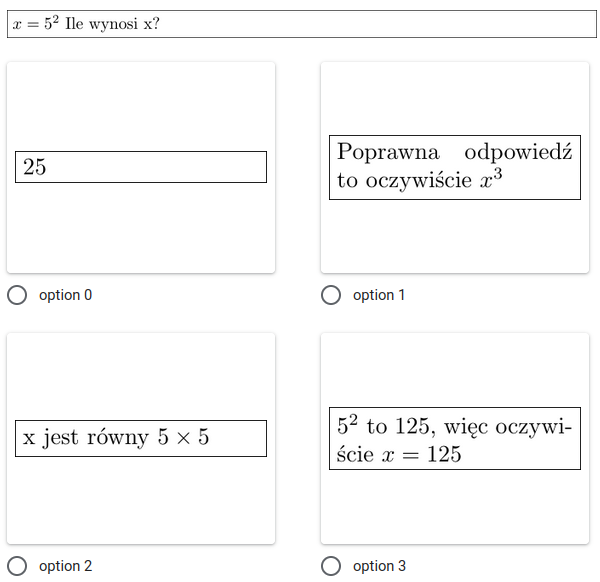
\includegraphics[scale=0.50]{odpowiedzi.png}
   \caption{Wygląd przykładowego formularza}
   \label{fig:1}
 \end{figure}
Dwie odpowiedzi zawsze zostaną umieszczona obok siebie, więc pliki graficzne z odpowiedziami
muszą być wąskie. Inaczej tekst odpowiedzi byłby bardzo mały. Zmiana wyświetlania odpowiedzi
z plikami graficznymi jest na ten moment niemożliwa. Dlatego do skryptu Google został dopisany
inny sposób generacji plików graficznych z odpowiedziami do pytań.

\section{Interfejs użytkownika}
Kod źródłowy aplikacji implementującej interfejs użytkownika znajduje się w katalogu
\texttt{forms-app-ui}. Aplikacja używa środowiska React i została stworzona używając programu
\texttt{Create React App}. Pliki \texttt{index.tsx} oraz \texttt{index.html}
tworzą podstawę całej aplikacji. W pliku \texttt{index.tsx} jest wstrzykiwany Reactowy
komponent \texttt{App}, który jest głównym komponentem całej aplikacji. W katalogu 
\texttt{src/components} można znaleźć wszystkie inne komponenty, które tworzą aplikację:
\begin{itemize}
  \item \texttt{FormCard}: implementuje jeden wpis z informacjami o formularzu,
  \item \texttt{FormList}: implementuje listę formularzy, czyli listę komponentów FormCard,
  \item \texttt{CreateDialog}: dialog, za pomocą którego można stworzyć nowy formularz,
  \item \texttt{AddDialog}: dialog, za pomocą którego można dodać już istniejący formularz,
  \item \texttt{EditDialog}: dialog, za pomocą którego można edytować formularz.
\end{itemize}
Aplikacja używa komponentów funkcyjnych oraz Reactowych hooków takich jak \texttt{useState},
\texttt{useEffect} i \texttt{useMemo}. W katalogu \texttt{src/models} znajdują się interfejsy
reprezentujące modele danych przesyłanych z serwera:
\begin{itemize}
  \item \texttt{AnswerTemplate}: jedna odpowiedź do pytania w formularzu,
  \item \texttt{QuestionTemplate}: jedno pytanie w formularzu,
  \item \texttt{FormTemplate}: formularz.
\end{itemize}
Dodatkowo znajduje się tam typ wyliczeniowy \texttt{QuestionType} z typami pytań.

\subsection{Material UI}
Implementacja korzysta z wiele komponentów z biblioteki Material UI takich jak:
\begin{itemize}
  \item \texttt{Alert} i \texttt{Collapse}, żeby wyświetlić ewentualne błędy,
  \item kontenery \texttt{List}, \texttt{ListItem}, \texttt{Box}, \texttt{Stack},
    \texttt{Accordion}, \texttt{Card},
  \item \texttt{Button}, żeby w łatwy sposób zaimplementować przyciski
    i ich logikę,
  \item \texttt{CircularProgress}, żeby wyświetlić animację ładowania, kiedy
    użytkownik musi poczekać na zakończenie jakiejś operacji,
  \item \texttt{Typography}, żeby wyświetlić tekst,
  \item \texttt{Dialog}, żeby zaimplementować dialogi,
  \item ikony.
\end{itemize}
Wszystkie te komponenty są niezwykle proste w użyciu oraz wyglądają przejrzyście
i łatwo do zrozumienia.
\subsection{Code Block}
Jeszcze jednym ważnym komponentem jest \texttt{CodeBlock} z biblioteki react-code-blocks.
Pozwala on łatwo wyświetlać fragmenty kodu razem z numerami linii i kolorowaniem
tekstu w zależności od języka kodu. Jest on wykorzystywany w komponencie FormCard.
\subsection{Daty}
Narzędzie pozwala określać rozpoczęcie i zakończenia testu, więc należało
zaimplementować zarządzanie datami. Aplikacja używa do tego biblioteki date-fns,
która jest lekka i prosta w użyciu. Przykładowo używamy funkcji \texttt{format}, żeby
ładnie wyświetlić daty we wpisach o formularzach.

\subsection{ESLint}
Podobnie jak w serwerze, tutaj również został użyty ESLint. W pliku
\texttt{.eslintrc.json}~zostały określone zasady dla projektu korzystającego
z języka TypeScript oraz środowiska React.

\section{Vagrant i Ansible}
Plik \texttt{Vagrantfile} służy do konfiguracji maszyny wirtualnej i środowiska,
na której będzie działać narzędzie. Wyjaśnię teraz krótko, jak działa ten 
skrypt. Pole \texttt{config.vm.box} określa jaki system operacyjny zostanie
użyty, w naszym przypadku jest to Ubuntu 20.04.4 LTS (Focal Fossa). 
Następnie skrypt instaluje Ansible i definiuje ścieżkę do playbooka Ansible,
który jest opisany w dalszej części tego rozdziału. W następnej części
udostępniamy porty na maszynie wirtualnej przez porty na systemie, na którym
działa ta maszyna.
\begin{verbatim}
  config.vm.network :forwarded_port, guest: 80, host: 8001
\end{verbatim}
W powyższym przykładzie udostępniamy port 8001 na maszynie wirtualnej
przez port 80 na systemie użytkownika. Dalej skrypt konfiguruje pamięć, którą
będzie mogła wykorzystać maszyna wirtualna i na końcu wypisuje wiadomość z adresami,
które należy odwiedzić po jej uruchomieniu. Przydatne polecenia:
\begin{itemize}
  \item \texttt{vagrant up}: uruchamia maszynę wirtualną,
  \item \texttt{vagrant halt}: zatrzymuje maszynę wirtualną,
  \item \texttt{vagrant reload}: resetuje maszynę wirtualną,
  \item \texttt{vagrant destroy}: usuwa maszynę wirtualną,
  \item \texttt{vagrant provision}: przeprowadza od początku proces konfiguracji
    maszyny razem z ponownym zainstalowaniem zależności z playbooka Ansible.
\end{itemize}

\subsection{Playbook}
Playbook to plik w formacie yaml, który określa jakie programy i biblioteki
powinny zostać zainstalowane oraz jakie usługi powinny zostać uruchomione po
uruchomieniu maszyny wirtualnej. Można go znaleźć w katalogu \texttt{playbooks}
pod nazwą \texttt{playbook.yaml}. Są w nim określone wszystkie programy
i biblioteki opisane w rozdziale ,,Środowisko'' oraz są w nim dodane polecenia
uruchomienia usług przez menadżera systemu \texttt{systemd}. Te usługi uruchamiają
aplikacje serwera oraz interfejsu użytkownika i ich konfigurację można znaleźć
odpowiednio w plikach \texttt{forms-app.service} i \texttt{forms-app-ui.service}.

\chapter{Instrukcja użytkownika}
\section{Początki pracy  z narzędziem}
Zanim zacznie się pracować z narzędziem, należy zainstalować
wszystkie wykorzystywane przez nie zależności. Instalacja została 
usprawniona wykorzystując Vagrant oraz Ansible, ale można ją przeprowadzić
również bez tych technologii. Oba te sposoby oraz późniejsza praca z narzędziem,
która zależy od wybranego sposobu instalacji są opisane poniżej.

\subsection{Projekt na Google Cloud}
Aplikacja używa Google Forms API do zarządzania formularzami na dysku Google
użytkownika i z tego powodu potrzebuje danych uwierzytelniających do 
komunikacji z tym API. Można je uzyskać zakładając projekt na Google Cloud.
Dokładne instrukcje można znaleźć w poradnikach w dokumentacji Google, 
a w tej pracy spróbuję krótko opisać ten proces: 

\begin{itemize}
  \item zaloguj się do konsoli Google Cloud,
  \item znajdź przycisk ,,Wybierz Projekt'',
  \item w nowym oknie naciśnij przycisk ,,Nowy Projekt'',
  \item wpisz nazwę projektu oraz lokalizację, a następnie naciśnij ,,Utwórz'',
  \item w menu po lewej stronie wybierz ,,Wyświetl Wszytskie Usługi'',
  \item w sekcji ,,Zarządzanie'' wybierz ,,Interfejsy API i usługi'',
  \item wybierz swój projekt,
  \item kliknij ,,Interfejsy API i usługi'',
  \item wyszukaj ,,Google Forms API'',
  \item w szczegółach Google Forms API kliknij ,,Włącz'',
  \item w menu po lewej stronie wybierz ,,Dane logowania'',
  \item kliknij ,,Create Credentials'', a potem ,,Klucz interfejsu API'',
  \item zapisz klucz w pliku i zachowaj na później,
  \item ponownie kliknij ,,Create Credentials'', a potem 
  ,,Identyfikator Klienta OAuth'',
  \item kliknij ,,Skonfiguruj Ekran Zgody'',
  \item jako typ użytkownika wybierz ,,Zewnętrzny'' i kliknij ,,Utwórz'',
  \item wpisz nazwę aplikacji, adresy e-mail i kliknij ,,Zapisz i kontynuuj'',
  \item kliknij ,,Dodaj lub usuń zakres'',
  \item w ,,Filtruj'' wpisz ,,Google Forms API'',
  \item zaznacz zakresy ,,forms.body'' i ,,forms.responses.readonly'',
  \item kliknij ,,Zaktualizuj'', następnie ,,Zapisz i kontynuuj'',
  \item dodaj swój adres konta Google do użytkowników testowych, kliknij
  ,,Zapisz i kontynuuj'' i na końcu ,,Powrót do panelu'',
  \item wybierz ponownie ,,Dane Logowania'', ,,Create Credentials''
  i ,,Identyfikator Klienta OAuth''
  \item jako typ aplikacji wybierz ,,Aplikacja internetowa'', dodaj URI 
  \\ \texttt{http://localhost:3000/oauth2callback} do sekcji ,,Autoryzowane 
  identyfikatory URI przekierowania'' i kliknij ,,Utwórz'',
  \item wybierz ,,Pobierz JSON''.
\end{itemize}

\subsection{Imgur API}
Aplikacja używa Imgur API, żeby wygenerować linki zewnętrzne obrazków
z formułami matematycznymi, z których pobiera je serwer Google. Do komunikacji
z Imgur API również potrzebujemy danych uwierzytelniania:
\begin{itemize}
  \item zaloguj się do Imgur,
  \item odwiedź stronę \href{https://api.imgur.com/}{Imgur API}
  \item znajdź ,,Register an application'',
  \item wypełnij dane, jako typ autoryzacji wybierz ,,OAuth2 authorization without
  a callback URL'',
  \item skopiuj Client ID i Client secret i zachowaj na później
\end{itemize}

\subsection{Repozytorium}
Teraz należy sklonować \href{https://github.com/arozkrut/forms-apps}
{repozytorium projektu} --- github.com/arozkrut/forms-app.
Następnie w pobranym repozytorium w katalogu \texttt{forms-app/src/credentials}
stwórz pliki:
\begin{itemize}
  \item \texttt{api\_key.txt}: wklej tu klucz interfejsu API, tak żeby plik był
  postaci
  \begin{verbatim}
    key=<uzyskany klucz>
  \end{verbatim}
  \item \texttt{credentials.json}: wklej tu zawartość pobranego pliku JSON,
  \item \texttt{imgur\_credentials.txt}: wklej tu Client ID i Client secret,
  tak żeby plik był postaci
  \begin{verbatim}
    ClientID: <Client ID>
    ClientSecret: <Client secret>
  \end{verbatim}
\end{itemize}

\subsection{Instalacja z Vagrant}
Jeśli masz już zainstalowany Vagrant wystarczy, że w głównym katalogu projektu
(tym z \texttt{Vagrantfile}) użyjesz polecenia \texttt{vagrant up}. Skrypt
Ansible zainstaluje wszystkie potrzebne zależności i uruchomi wszystkie
aplikacje. Ważne jest, że projekt potrzebuje portów 3000, 9090 i 9091.
Jeśli któryś z nich jest już zajęty narzędzie nie uruchomi się. Instalacja może
chwilę potrwać. Po jej zakończeniu wyświetli się wiadomość z linkiem prowadzącym
do strony uwierzytelniania Google, gdzie trzeba wybrać konto Google, na którym
będą przechowywane formularze oraz wyrazić zgodę na nadanie aplikacji dostępu do
formularzy na tym koncie Google. Następnie w przeglądarce należy odwiedzić adres
\href{http://localhost:9091}{http://localhost:9091}, gdzie działa interfejs
użytkownika. Narzędzie jest gotowe do pracy.

\subsection{Instalacja bez Vagrant}
Jeśli użytkownik chce korzystać z narzędzia bez zainstalowanego Vagrant, musi on
sam zainstalować wszystkie zależności: Python 3, \LaTeX{}, poppler-utils, biblioteki
do języka Python opisane w poprzednim rozdziale, nodejs, npm. Następnie w katalogach
\texttt{forms-app} oraz \texttt{forms-app-ui} należy wydać polecenie \texttt{npm i}.
Teraz należy włączyć serwer NodeJS poleceniem \texttt{node src/server.js} 
(koniecznie w katalogu \texttt{forms-app}). W przeglądarce powinna uruchomić się
strona uwierzytelniania Google, gdzie trzeba wybrać konto Google, na którym
będą przechowywane formularze oraz wyrazić zgodę na nadanie aplikacji dostępu do
formularzy na tym koncie Google. Po tym w katalogu \texttt{src/forms-app-ui}
należy włączyć serwer interfejsu użytkownika poleceniem \texttt{npm start}, który
uruchomi się pod adresem \href{http://localhost:9091}{http://localhost:9091}.
Po odwiedzeniu tej strony w przeglądarce można zacząć pracować z narzędziem.

\section{Praca z narzędziem}

\subsection{Schemat pliku kodującego (JSON)}
Poniżej znajduje się rozpisany schemat kodowania: 
\begin{figure}[H]
\begin{lstlisting}[language=json,firstnumber=1]
{
  "title": "string",
  "description: "string",
  "startDate": "string",
  "endDate": "string",
  "shuffleAnswers": "boolean",
  "questions": [{
    "type": "string", 
    "text": "string",
    "tex" : "boolean",
    "answers": [{
      "text" : "string",
      "tex" : "boolean",
      "correct" : "boolean"
    }],
    "points": "number"
    "pointsArray": "array"
  }]
}

\end{lstlisting}
\end{figure}
Jest to opis tych wartości, które mogą być użyte --- nie wszystkie są jednak 
wymagane. Poniżej znajduje się szczegółowy opis pól i wartości:
\begin{itemize}
  \item{title} -- wartość tekstowa, odpowiada nagłówkowi formularza --- 
  \textbf{pole wymagane},
  \item{description} -- wartość tekstowa, krótki opis formularza, który
  pojawi się pod tytułem ---  \textbf{pole opcjonalne},
  \item{startDate} -- wartość tekstowa, data planowanego rozpoczęcia testu
  w formacie ISO. To pole służy tylko do odrzucania odpowiedzi, które zostały
  przesłane przed podaną datą podczas oceniania ---  \textbf{pole opcjonalne},
  \item{endDate} -- wartość tekstowa, data planowanego zakończenia testu
  w formacie ISO. To pole służy tylko do odrzucania odpowiedzi, które zostały
  przesłane po podanej dacie podczas oceniania ---  \textbf{pole opcjonalne},
  \item{shuffleAnswers} -- wartość boolowska, informacja o tym, czy odpowiedzi
  dla każdego pytania powinny zostać przetasowane dla każdego wyświetlenia
  formularza. Niestety na ten moment Google Forms API nie udostępnia opcji
  tasowania pytań, można ją jedynie włączyć ręcznie w ustawieniach formularza
  na stronie Google: settings -> presentation -> Shuffle question order
  ---  \textbf{pole opcjonalne},
  \item{questions} -- tablica, której każde pole zawiera informacje dotyczące
  jednego pytania --- \textbf{pole wymagane}. \\Poniżej znajdują się wartości
  kodujące pojedyncze pytanie:
  \begin{itemize}
    \item{type} -- pole tekstowe dotyczące typu kodowanego pytania.
    Dopuszczalne wartości:
    \begin{itemize}
      \item ,,checkBox'' -- pytanie zamknięte wielokrotnego wyboru,
      \item ,,grid'' -- pytanie typu ,,prawda/fałsz'',
      \item ,,list'' -- zamknięte jednokrotnego wyboru,
      \item ,,text'' -- otwarte.
    \end{itemize}
    \textbf{pole wymagane},
    \item{text} -- zawiera treść pytania w formie tekstowej. Może zawierać wstawki
    z \LaTeX{}'a. Należy jednak pamiętać, że JavaScript traktuje symbol ,,$\backslash$''
    jako specjalny --- wszystkie wystąpienia ,,$\backslash$'' należy więc zastąpić
    ,,$\backslash\backslash$'' --- \textbf{pole wymagane},
    \item{tex} -- wartość boolowska, jeśli \textbf{true} treść pytania (text) będzie
    konwertowana do obrazu z zachowaniem konwersji symboli matematycznych i innych
    wstawek z \LaTeX{}'a z biblioteki standardowej --- \textbf{pole wymagane},
    \item{answers} -- tablica, każde pole zawiera jedną z możliwych odpowiedzi w
    następującej formie:
    \begin{itemize}
      \item text -- pole tekstowe, treść danej odpowiedzi,
      \item tex -- wartość boolowska, jeśli \textbf{true} treść odpowiedzi (text) będzie
      konwertowana do obrazu z zachowaniem konwersji symboli matematycznych i innych
      wstawek z \LaTeX{}'a z biblioteki standardowej, tylko dla pytań typu list i checkBox,
      \item correct -- wartość boolowska wskazująca czy dana odpowiedź jest prawidłowa.
      Domyślna wartość: false.
    \end{itemize} 
    --- \textbf{pole opcjonalne},
    \item{points} -- wartość numeryczna, odpowiada liczbie punktów przyznawanej za
    poprawą odpowiedź na pytanie (tylko dla pytań typu list)
    --- \textbf{pole opcjonalne},
    \item{pointsArray} -- tablica z wartościami numeryczymi, odpowiada liczbie punktów
    przyznawanej za poprawne odpowiedzi na pytanie (tylko dla pytań typu checkBox i grid),
    przykładowo wartość $ [0, 1, 3] $ wskazuje, że jeśli nie zostanie wybrana żadna dobra
    odpowiedź, zostanie przyznane 0 punktów, jeśli zostanie udzielona jedna dobra odpowiedź,
    zostanie przydzielony 1 punkt i jeśli zostaną udzielone dwie dobre odpowiedzi, zostaną
    przydzielone 3 punkty
    --- \textbf{pole opcjonalne}
  \end{itemize}
\end{itemize}

\subsection{Automatyczne ocenianie}
Pytania typu list, checkBox i grid mogą zostać automatycznie ocenione i wyniki mogą zostać
pobrane w formacie JSON lub pliku Excel. Jeśli chcemy, żeby odpowiedzi zostały ocenione
musimy ręcznie ustawić zbieranie adresów email w ustawieniach formularza. Google Forms API
niestety na ten moment nie udostępnia możliwości zrobienia tego automatycznie. Sposób
oceniania zależy od typu pytania:
\begin{itemize}
  \item \textbf{list}: jeśli zostanie zaznaczona poprawna odpowiedź, odpowiadający uzyska
  całość punktów z pola \texttt{points}, w przeciwnym przypadku otrzyma 0 punktów,
  \item \textbf{checkBox}: zliczane są poprawnie zaznaczone odpowiedzi i od tej liczby
  odejmuje się liczbę niepoprawnie zaznaczonych odpowiedzi. Jeśli uzyskana liczba jest
  mniejsza od zera, podstawiamy za nią 0. Następnie z tablicy
  \texttt{pointsArray} z indeksu równego poprzednio uzyskanej liczbie odczytuje się liczbę
  uzyskanych punktów,
  \item \textbf{grid}: zliczane są poprawnie udzielone odpowiedzi i z indeksu równego
  tej liczbie odczytuje się liczbę uzyskanych punktów w tablicy \textbf{pointsArray}.
\end{itemize} 

\subsection{Obsługa narzędzia}
Po uruchomieniu użytkownik widzi stronę w przeglądarce, jak na zdjęciu poniżej:
\begin{figure}[H]
 \centering
  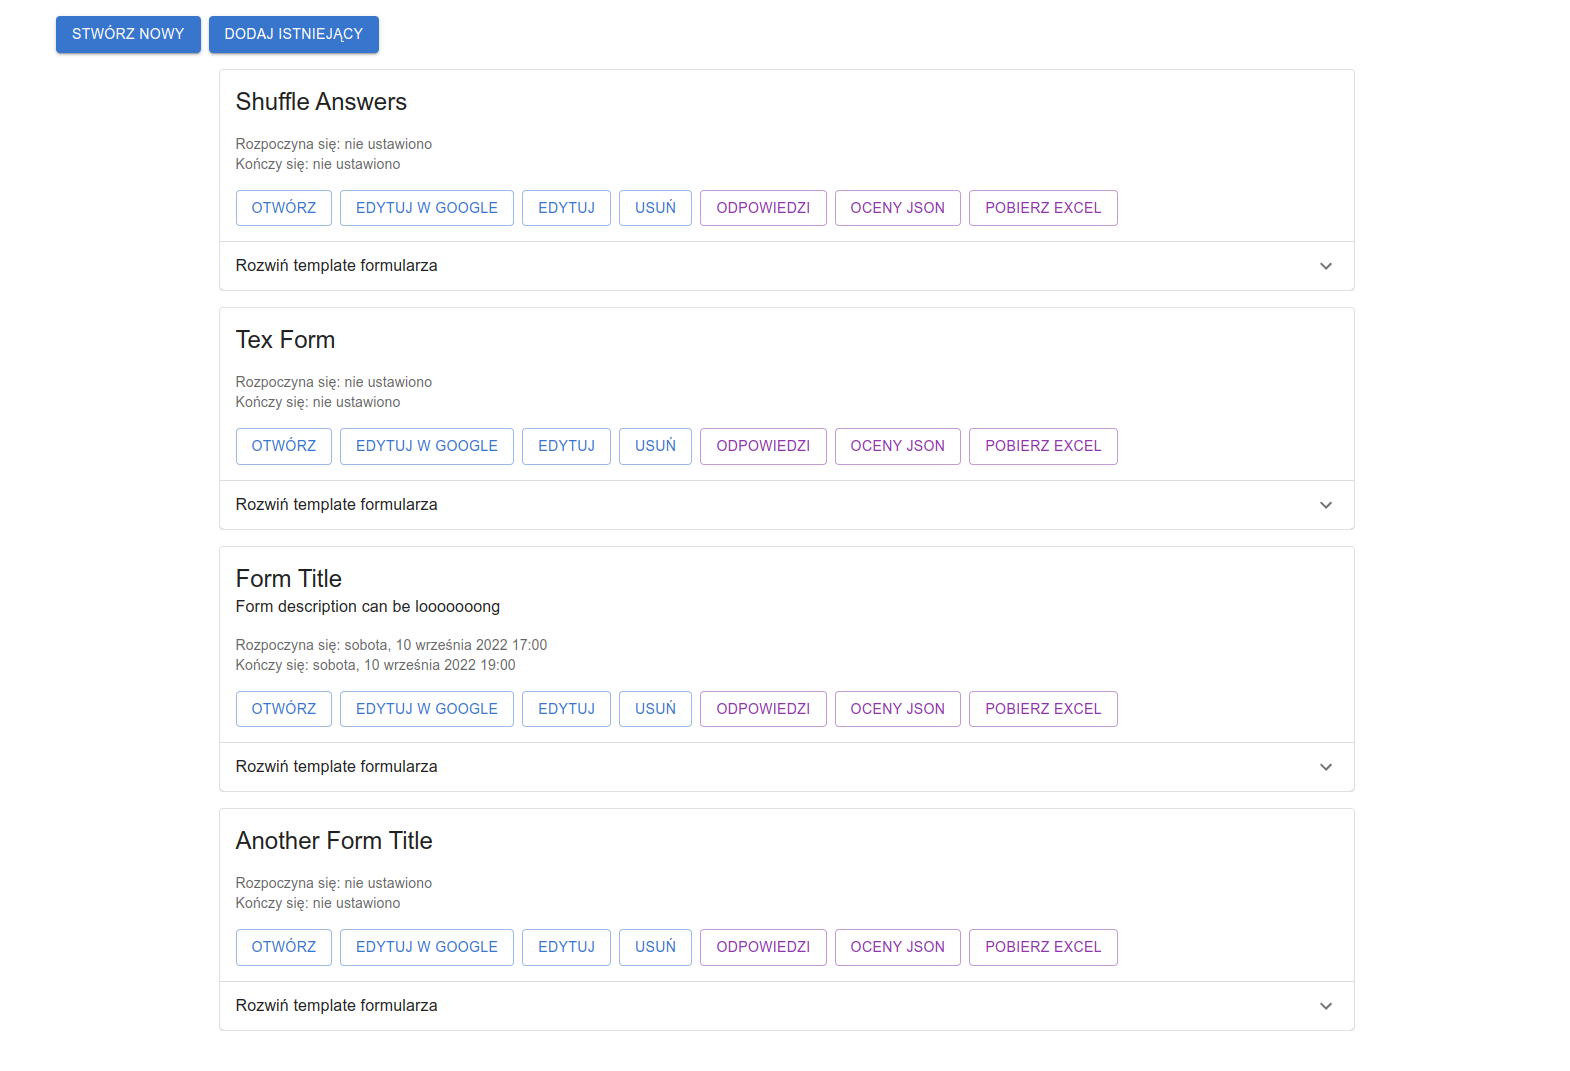
\includegraphics[scale=0.30]{strona.png}
  \caption{Interfejs aplikacji}
  \label{fig:1}
\end{figure}
Przycisk ,,Stwórz nowy'' otworzy dialog, w którym należy wprowadzić kodowanie 
formularza i ewentualnie czas rozpoczęcia i zakończenia testu. Po kliknięciu 
,,Stwórz'' na dysku Google zostanie stworzony nowy formularz i wpis o nim pojawi
się na liście na głównej stronie aplikacji. Przycisk ,,Dodaj istniejący'' otworzy
dialog, gdzie możemy podać identyfikator istniejącego już formularza, który chcemy
dodać do listy formularzy zarządzanych przez aplikację. Musimy również podać jego
kodowanie. Po kliknięciu ,,Dodaj'' formularz zostanie zedytowany i pojawi się na 
liście formularzy. Na liście formularzy każdy wpis odpowiada jednemu formularzowi
na dysku Google użytkownika, jednak nie wszystkie formularze na dysku się tu pojawią,
jedynie te stworzone przez aplikację lub dodane używając przycisku ,,Dodaj istniejący''.
W każdym wpisie możemy znaleźć przyciski:
\begin{itemize}
  \item ,,Otwórz'': otwiera formularz na stronie Google w nowej karcie,
  \item ,,Edytuj w Google'': otwiera stronę edycji formularza na stronie Google
    w nowej karcie,
  \item ,,Edytuj'': otwiera dialog, gdzie można edytowac kodowanie formularza,
  \item ,,Usuń'': usuwa formularz z listy formularzy zarządzanych przez aplikację
    i usuwa całą jego zawartość, jednak pusty formularz tylko z tytułem pozostanie 
    na dysku Google użytkownika,
  \item ,,Odpowiedzi'': pokazuje wszystkie przesłane odpowiedzi, łącznie z tymi
    przesłanymi przed początkiem lub po końcu ustawionych w kodowaniu formularza,
  \item ,,Oceny JSON'': wyświetla ocenione odpowiedzi bez pytań otwartych w formacie
    JSON,
  \item ,,Pobierz Excel'': pobiera plik Excel z ocenionymi zamkniętymi pytaniami,
  \item ,,Rozwiń template formularza'': podgląd kodowania formularza,
\end{itemize}

\subsection{Przeprowadzanie egzaminów}
Jeśli narzędzie ma byc użyte do przeprowadzenia egzaminu na początku należy stworzyć
z jego pomocą pusty formularz tylko z tytułem, ewentulanie krótką informacją o czasie
startu. Przed rozpoczęciem należy ręcznie włączyć w ustawieniach formularza na stronie
Google zbieranie adresów email i ewentualnie tasowanie pytań. Następnie w momencie
rozpoczęcia egzaminu należy go zaktualizować dodając do niego pytania.
Po czasie zakończenia egzaminu można go ręcznie zamknąć, ale jeśli ma zostać użyte
automatyczne ocenianie, nie wolno zmieniać jego kodowania w aplikacji. Narzędzie
przefiltruje przesłane odpowiedzi i automatycznie je oceni po kliknięciu
odpowiedniego przycisku.


\chapter{Podsumowanie}


\bibliographystyle{unsrt} %{abbrv} % unsrt sortuje według kolejności wystąpień
\bibliography{bibliografia}

\appendix

\end{document}
